\section{Software development methodology}
\subsection{Software Development Life Cycle}
\begin{figure}[h!]\centering
	\fbox{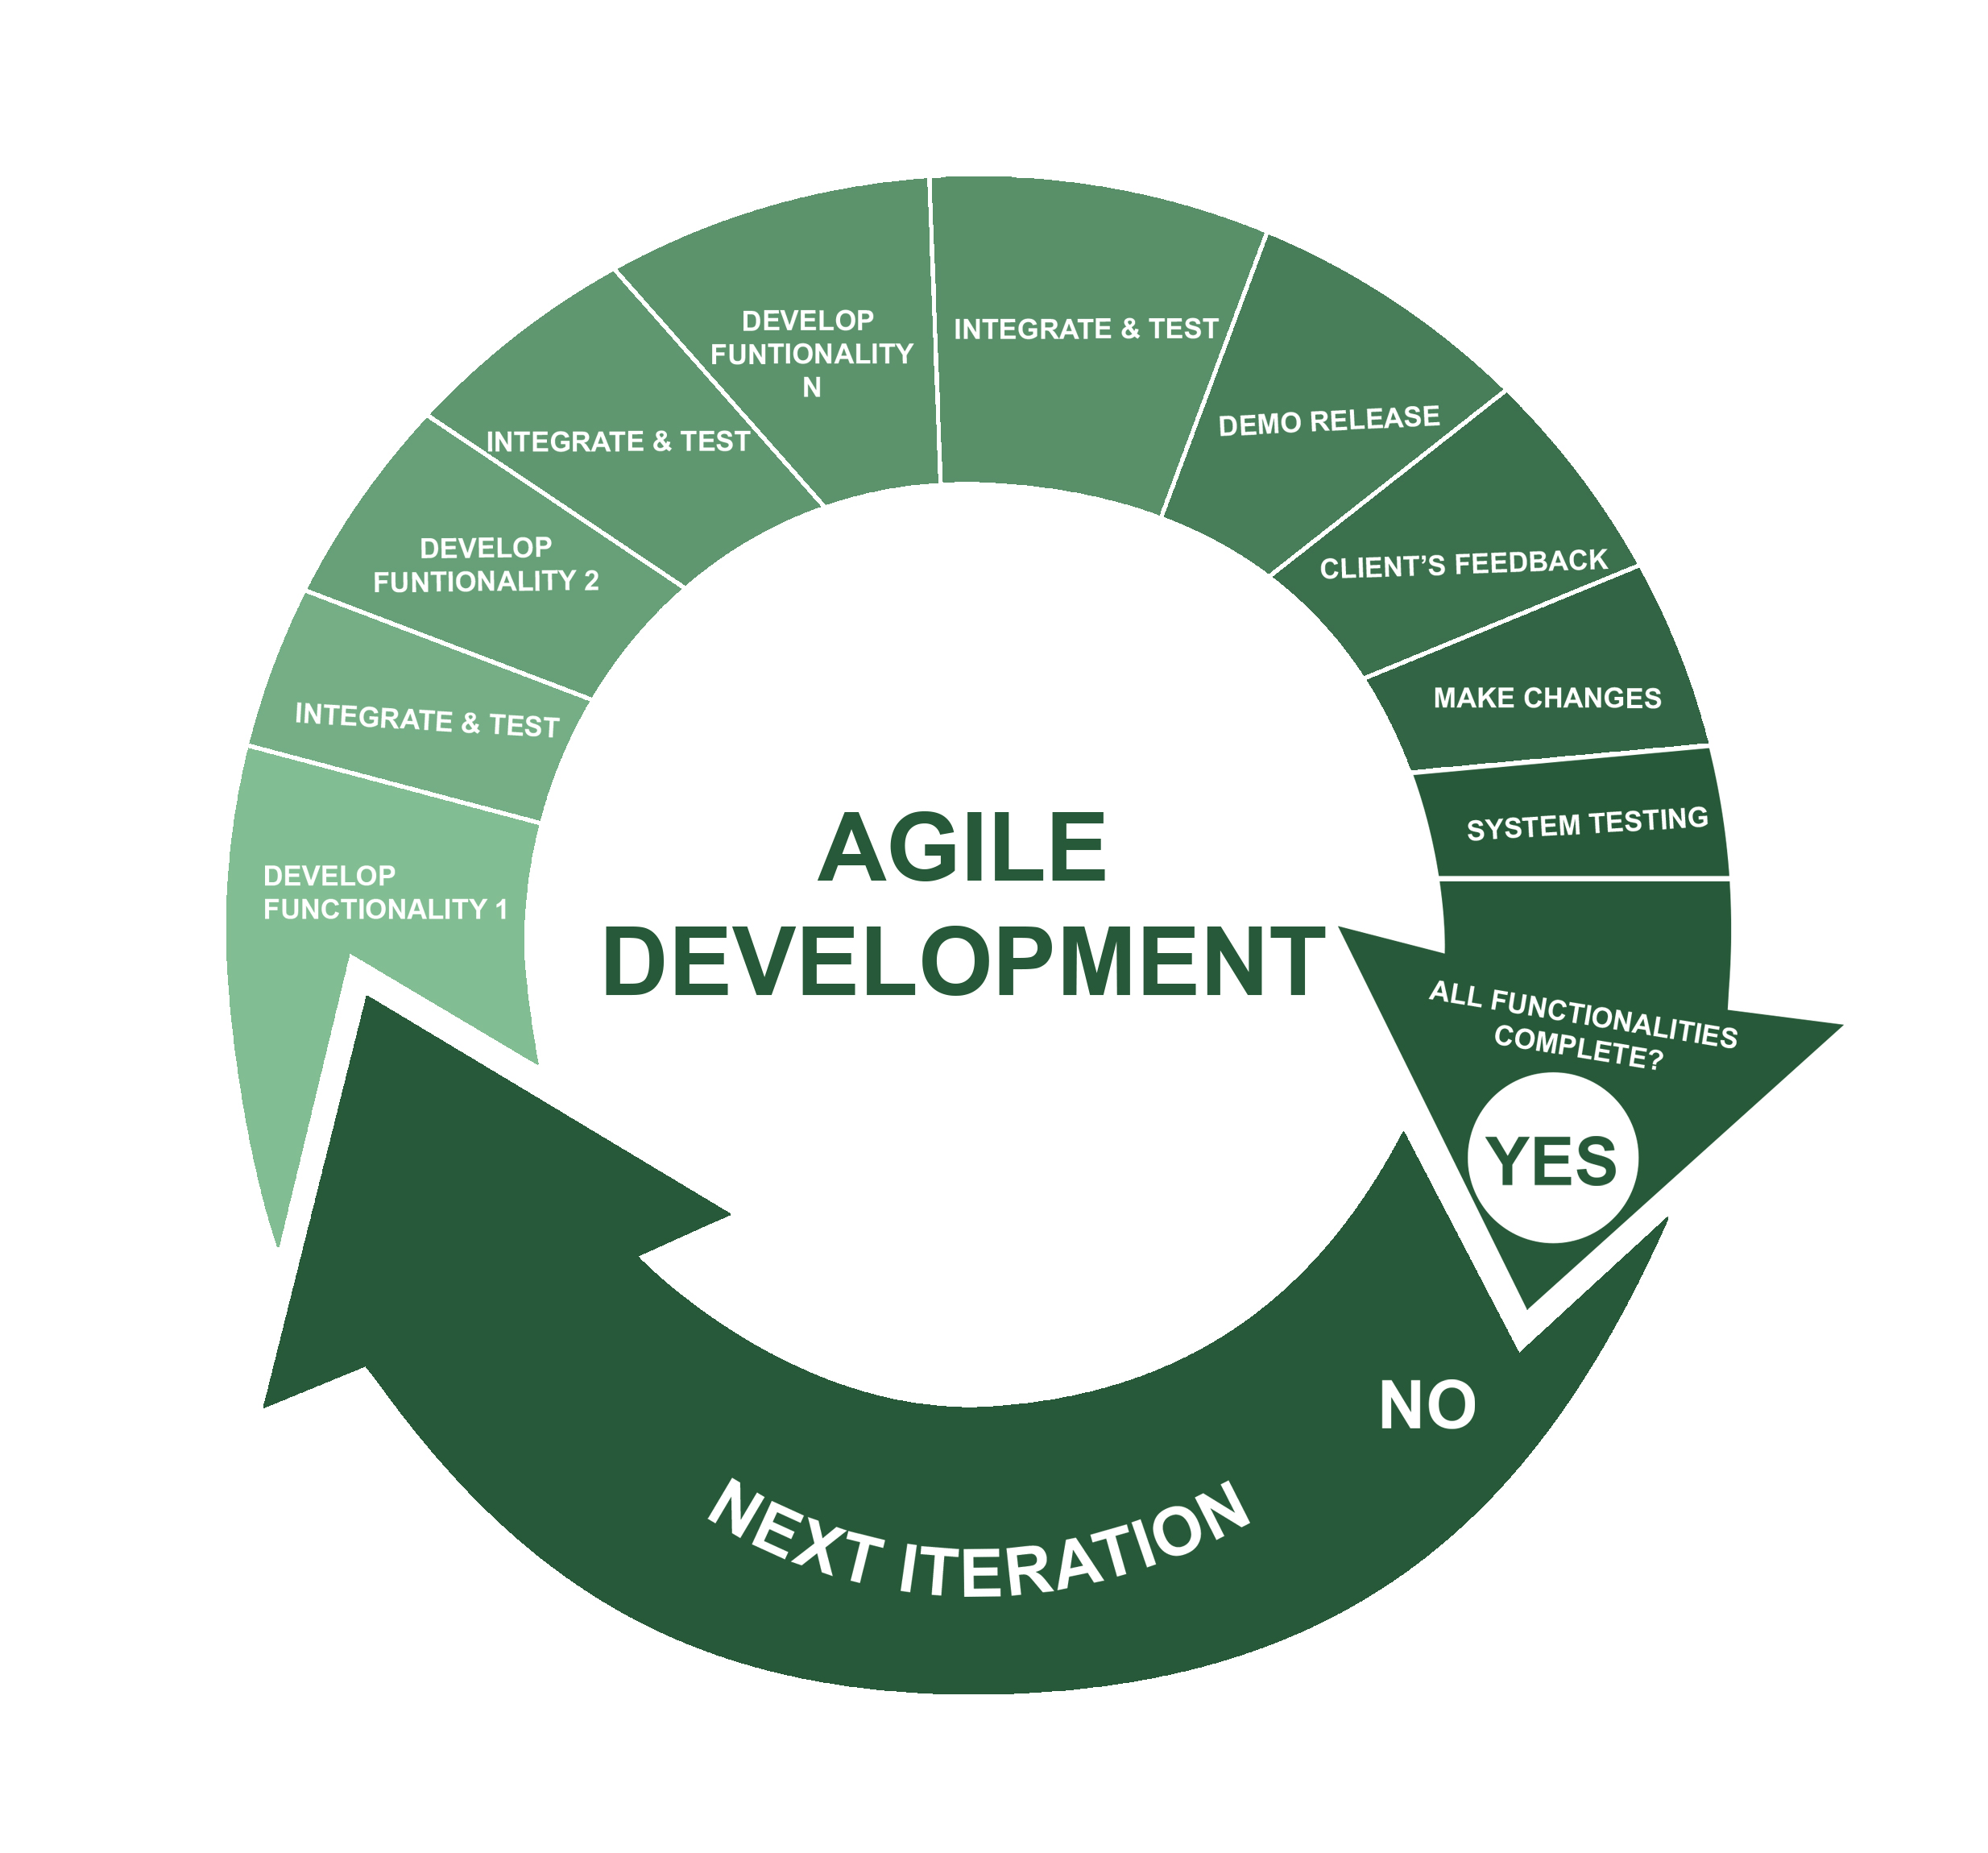
\includegraphics[width=4in]{fig/agile}}
	\caption{Agile Development Life Cycle}
	\label{fig:agile}
\end{figure}

For the project Agile software development life cycle was followed. \cite{ad} The Agile software development life cycle is based upon the iterative and incremental process models, and focuses upon adaptability to changing product requirements and enhancing customer satisfaction through rapid delivery of working product features and client participation. Agile methods primarily focus upon breaking up the entire product into smaller, easily developable, "shippable" product features developed through "incremental" cycles known as "sprints". Agile methodology is an alternative to traditional project management, typically used in software development. Agile methodologies are an alternative to waterfall, or traditional sequential development. Agile development model is a type of Incremental model. Software is developed in incremental, rapid cycles. This results in small incremental releases with each release building on previous functionality. Each release is thoroughly tested to ensure software quality is maintained. Agile model is generally used for time critical applications.

The Agile Manifesto is based on twelve principles :
\begin{itemize}
	\item Customer satisfaction by early and continuous delivery of valuable software
	\item Welcome changing requirements, even in late development
	\item Working software is delivered frequently (weeks rather than months)
	\item Close, daily cooperation between business people and developers
	\item Projects are built around motivated individuals, who should be trusted
	\item Face-to-face conversation is the best form of communication (co-location)
	\item Working software is the principal measure of progress
	\item Sustainable development, able to maintain a constant pace
	\item Continuous attention to technical excellence and good design
	\item Best architectures, requirements, and designs emerge from self-organizing teams
	\item Regularly, the team reflects on how to become more effective, and adjusts accordingly
\end{itemize}

The major characteristics of this model are listed below:
\begin{enumerate}
	\item Self-organisation and motivation takes precedence over delegation of authority and following the "seniority" hierarchy. The Agile team has to collaborate and share ideas to develop the product "as a whole" unit i.e. each member should support a common vision.
	\item Agile concentrates upon delivering sustained "working" product releases through product incremental cycles over documentation and working protocols. The main objective is to develop, and deliver, bug free product feature releases in a continuous and sustained manner until the entire product is developed.
	\item Agile focuses upon incorporating dynamic changes in the product development cycle. Changes in the product features can be easily and effortlessly carried out by developing "user stories"- product functionality or features as defined in the product backlog.
	\item Stakeholders and project owners "clear" the product features developed through the sprint cycles. A lot of time is saved through customer collaboration, and the project proceeds in a successful manner as the client always approves the development keeping in mind the current market trends.
\end{enumerate}

The project is started by preparing the backlog. The backlog contains the modular decomposition of the overall system. Then the requirement specification and system model diagrams are prepared. Agile is an adaptive model which allows continuous changes in the system requirements as well the system model.

\subsection{Requirement Analysis}
The functional and non-functional requirements of this project are as listed below.
\subsubsection{Functional Requirements}
\begin{itemize}
	\item The system shall examine the stocks of different companies based on the technical indicators, fundamental factors and news sentiments.
	\item The system shall predict the current value of a stock based on past values of that stock.
	\item The system shall predict the increase or decrease of the NEPSE index based on news analysis.
	\item The system shall predict the intrinsic worth of a company based on the fundamental indicators of the company.
	\item The system shall provide visualization of the stock market's data for individual companies of different sectors.
\end{itemize}

\subsubsection{ Non-Functional Requirements}
\begin{itemize}
	 \item The system must predict stock market with acceptable accuracy.  
	\item The data used for the prediction and analysis should be real and fault proof. Irregularities in data should be removed by using various techniques.
	\item The prediction system should be dynamic enough to easily adapt with the daily increase in the number of data.
	\item The visualization should be adaptive to dynamically add new data.
\end{itemize}

\subsection{Backlog}
The backlog of project is described in the table \ref{tab:Backlog}
{
	\renewcommand{\arraystretch}{1.5}
	\begin{table}
	\begin{tabular}{|p{3cm}|p{7cm}|p{2cm}|p{2cm}|}
	\hline
	{\bf Story} & {\bf Task} & {\bf Time Estimation(Days)} & {\bf Time Estimation(Hours)}\\
	\hline
	\multirow{6}{3cm}{As a user, I should have access to stock data} & Crawl data from Merolagani, Sharesansar and NEPSE website & 7 & 35\\
	\cline{2-4}
	& Clean the data obtained from the web & 1 & 5\\
	\cline{2-4}
	& Design a data model and represent the data in proper format & 7 & 35\\
	\cline{2-4}
	& CRUD on the available data set & 7 & 35\\
	\cline{2-4}
	& Design simple User Interface to view the stock data & 6 & 30\\
	\cline{2-4}
	& Perform Tests & 2 & 10\\
	\cline{2-4}
	\hline
	\multirow{5}{3cm}{As a user, I should be able to visualize the stock data for various companies and sector, compare and analyze them} & Represent data in proper format for visualization & 3 & 15\\
	\cline{2-4}
	& User Interface for data visualization & 3 & 15\\
	\cline{2-4}
	& Implementation of data visualization using Amcharts & 7 & 35\\
	\cline{2-4}
	& Design and write test cases & 4 & 20\\
	\cline{2-4}
	& Perform test & 1 & 5\\
	\cline{2-4}
	\hline
	\multirow{3}{3cm}{As a user, I should be able to view the fundamental background of a company} & Represent the fundamental data in proper format & 5 & 25\\
	\cline{2-4}
	& User Interface for viewing fundamental data & 4 & 20\\
	\cline{2-4}
	& Integrate back-end and front-end & 4 & 20\\
	\hline 
	\multirow{8}{3cm}{As a user I should be able to predict the company wise stock price} & Design a model of data for prediction & 7 & 35\	\
	\cline{2-4}
	& Design the prediction engine using ANN & 25 & 125\\
		\cline{2-4}
		& Implement the prediction engine & 15 & 75\\
	\cline{2-4}
	& Refine the ANN model & 5 & 25\\
	\cline{2-4}
	& Design the prediction engine using KNN & 5 & 25\\
	\cline{2-4}
	& Implement the prediction engine & 2 & 10\\
	\cline{2-4}	
	& Test the prediction engine & 2 & 10\\
	\hline
	\multirow{5}{3cm}{As a user I should be able to predict the nepse index} & Design a news data model for prediction & 10 & 50\\
	\cline{2-4}
	& Design a prediction using KNN & 5 & 25\\
	\cline{2-4}
	& Implement the prediction engine & 2 & 10\\
	\cline{2-4}
	& Test the prediction engine & 2 & 10\\
	\hline
	\end{tabular}
	\caption{Backlog}
	\label{tab:Backlog}

\end{table}
}

%\newpage
\subsection{System Design}
\subsubsection{System Architecture}
\begin{figure}[H]\centering
  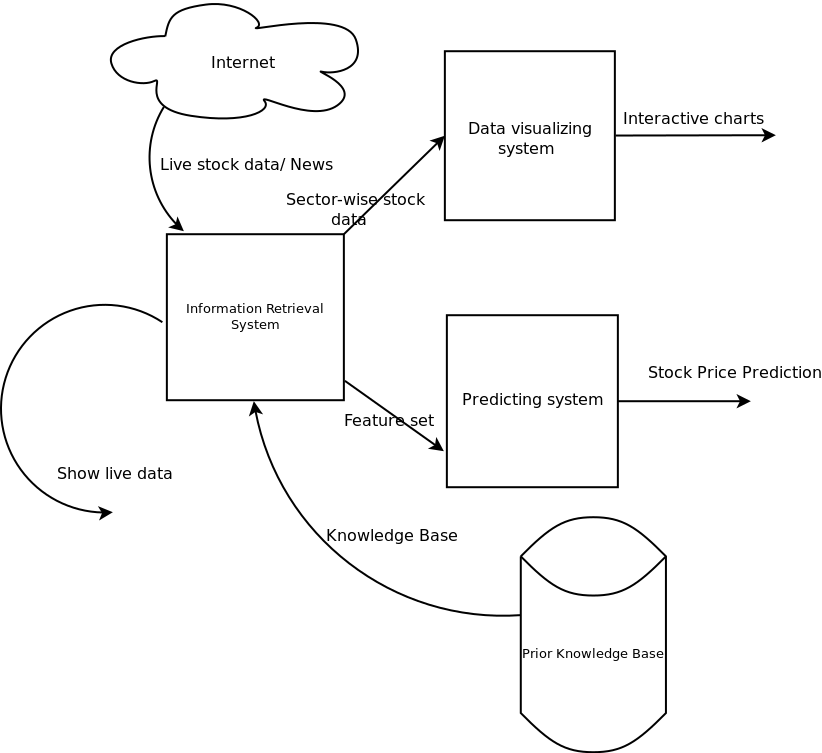
\includegraphics[width=5in]{fig/System}
  \caption{Overall system architecture}
  \label{fig:System}
\end{figure}

\subsubsection{UML Diagrams}
\begin{figure}[H]\centering
  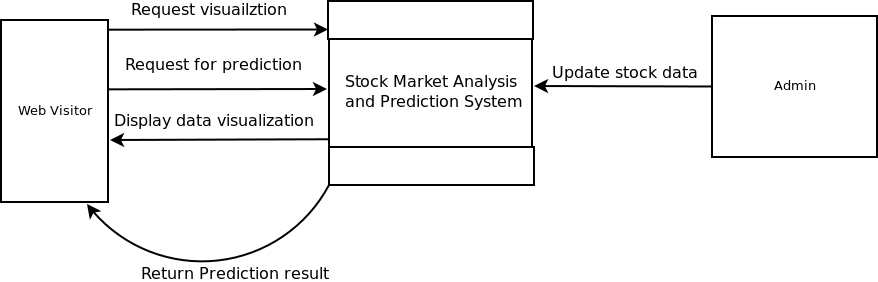
\includegraphics[width=6in]{fig/Dfd1}
  \caption{Level-1 dataflow diagram (DFD)}
  \label{fig:Dfd1}
\end{figure}

~

\begin{figure}[H]\centering
  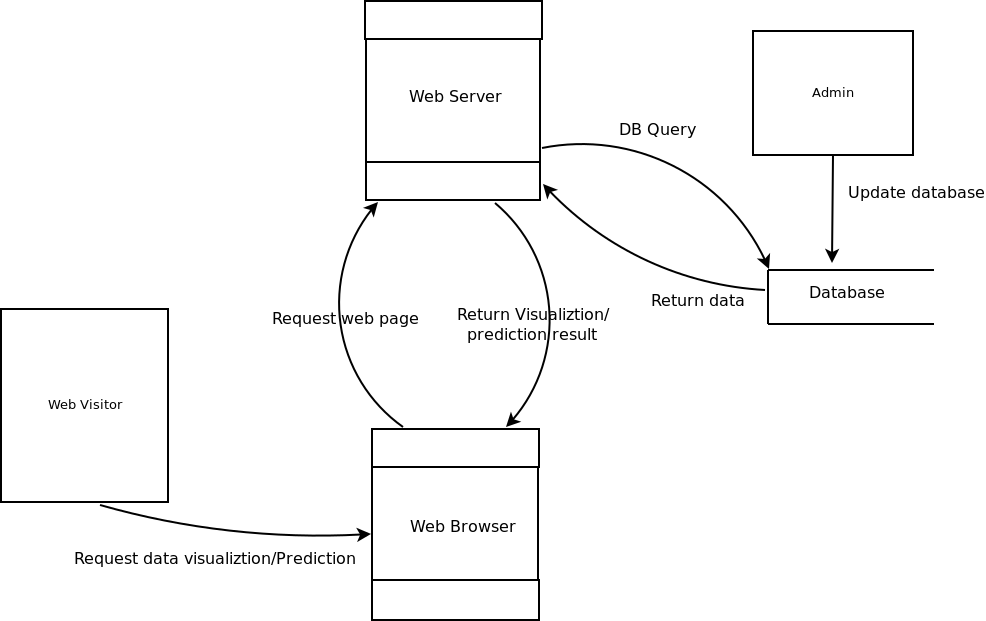
\includegraphics[width=6in]{fig/DFD2}
  \caption{Level-2 dataflow diagram (DFD)}
  \label{fig:DFD2}
\end{figure}


\begin{figure}[H]\centering
  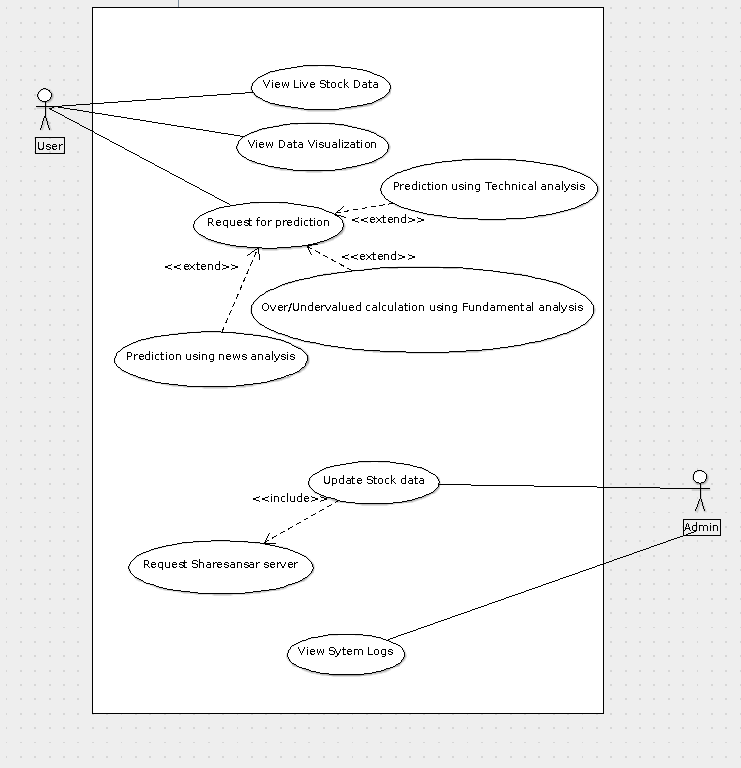
\includegraphics[width=6.5in]{fig/usecase2}
  \caption{Use case diagram}
  \label{fig:usecase2}
\end{figure}

\begin{figure}[H]\centering
  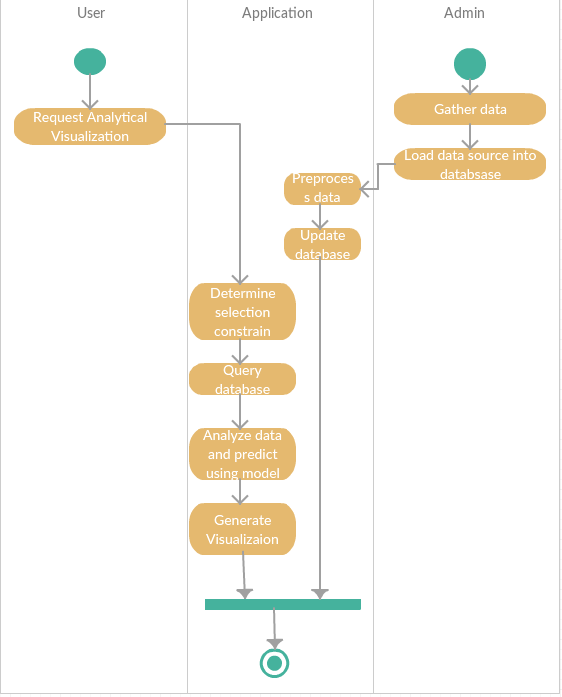
\includegraphics[width=6.5in]{fig/activity}
  \caption{Activity diagram}
  \label{fig:activity}
\end{figure}

\begin{figure}[H]\centering
  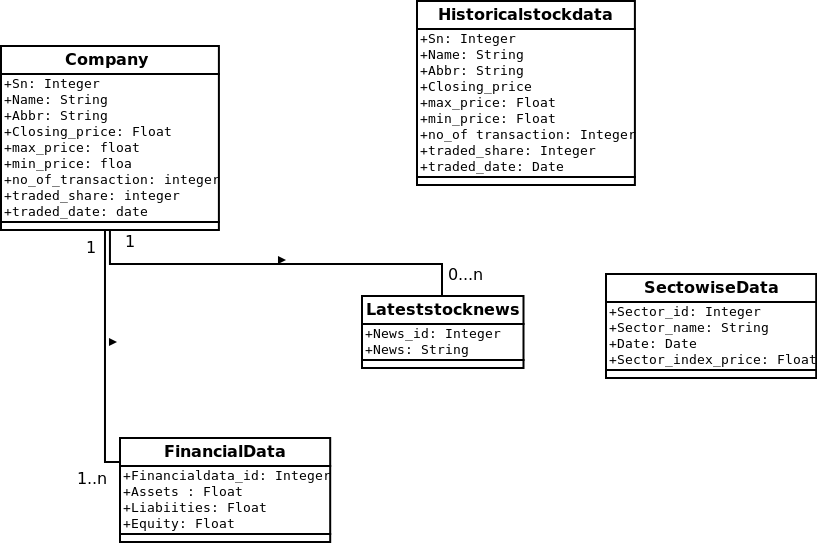
\includegraphics[width=6in]{fig/classdiagram}
  \caption{Class diagram}
  \label{fig:classdiagram}
\end{figure}

~

\begin{figure}[H]\centering
  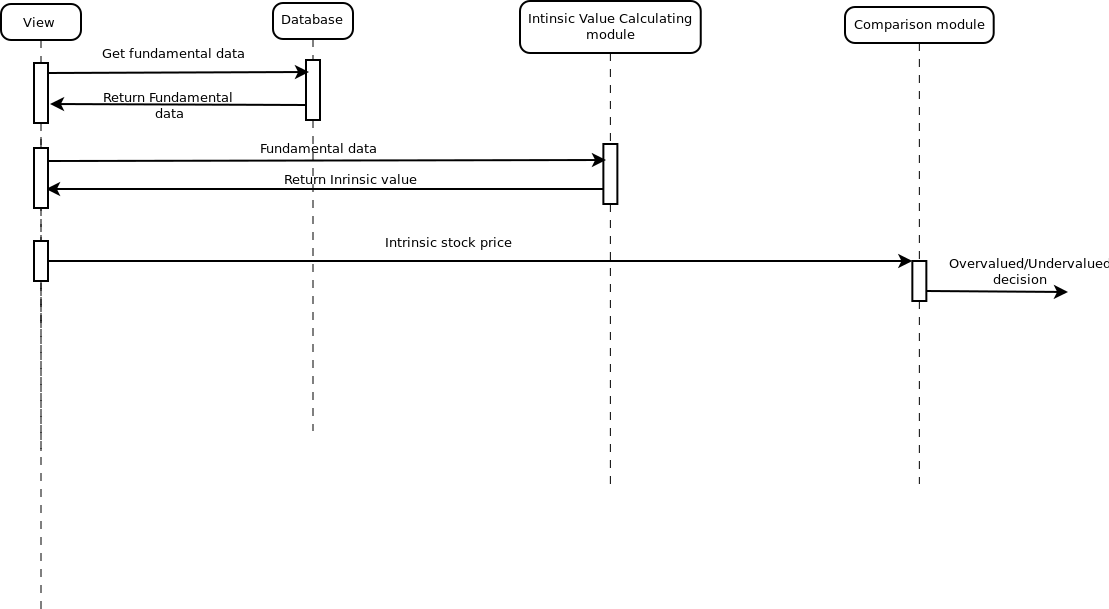
\includegraphics[width=\textwidth]{fig/fundamental}
  \caption{Sequence diagram for Fundamental Analysis}
  \label{fig:Fundamental}
\end{figure}

\begin{figure}[h!]
  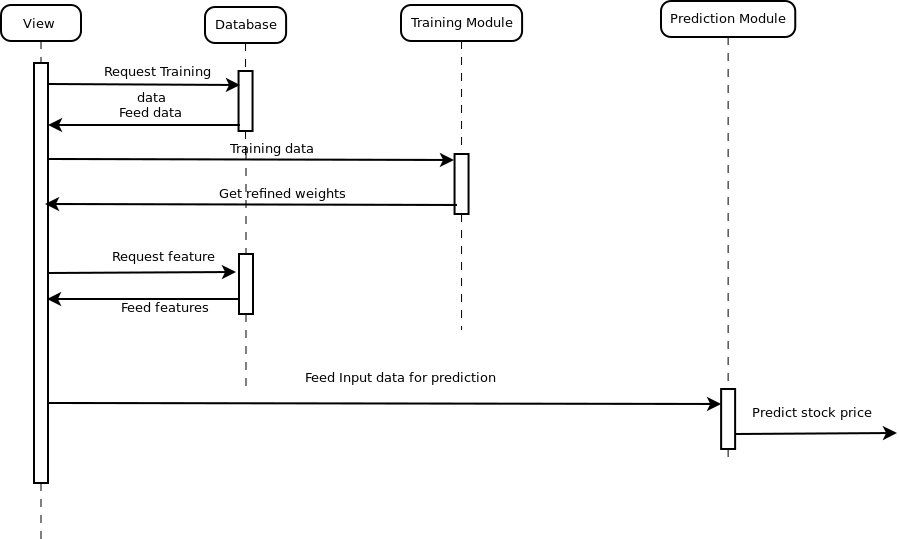
\includegraphics[width=\textwidth]{fig/StockPredictionusingNN}
  \caption{Sequence diagram For technical analysis using NN }
  \label{fig:StockPredictionusingNN}
\end{figure}

~


\begin{figure}[H]\centering
  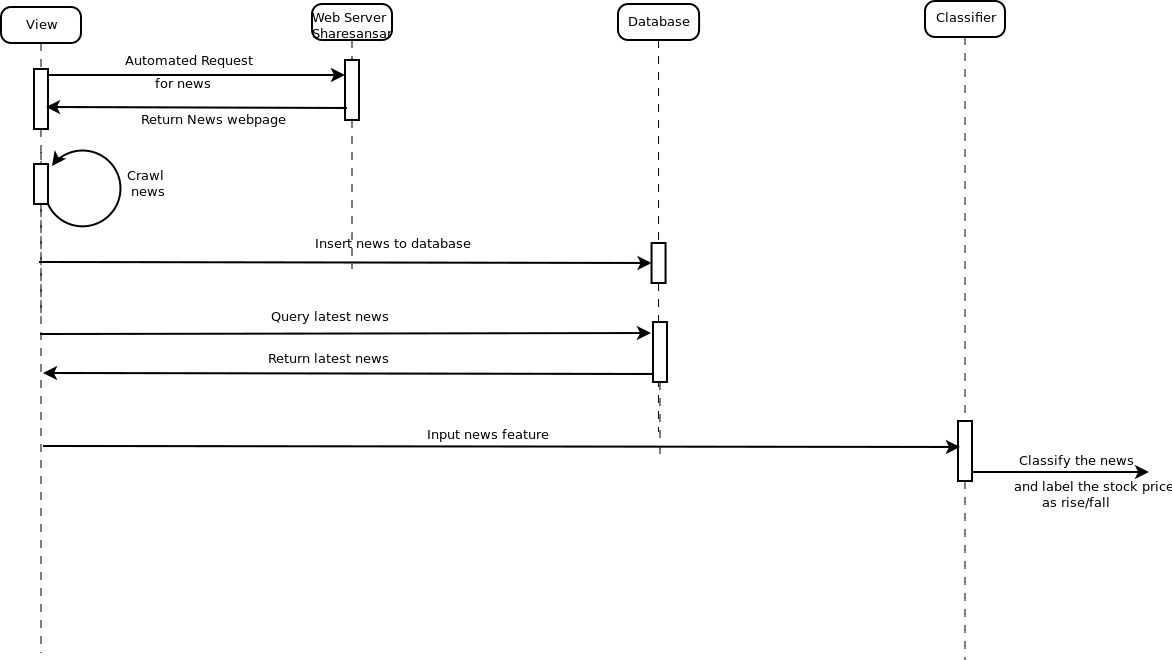
\includegraphics[width=6in]{fig/newsanalysis}
  \caption{Sequence diagram for New Analysis}
  \label{fig:newsanalysis}
\end{figure}

\begin{figure}[H]\centering
  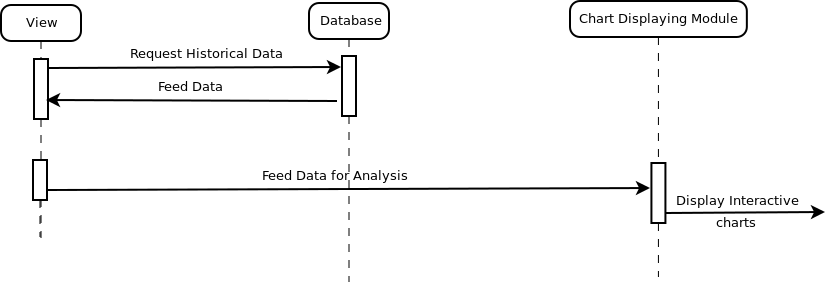
\includegraphics[width=6in]{fig/Charting}
  \caption{Sequence diagram for Data Visualization}
  \label{fig:Charting}
\end{figure}




%by anuj
\subsection{Tools and Technique}
The various tools and techniques used in this project are described below: 
%\subsubsection{Tools}
\subsubsection{Python}
The whole project is written in Python Programming Language. Various libraries of python are used in the project. Python is a general-purpose interpreted, interactive, object-oriented, and high-level programming language. It was created by Guido van Rossum during 1985- 1990. Like Perl, Python source code is also available under the GNU General Public License (GPL).

Python is designed to be highly readable. It uses English keywords frequently where as other languages use punctuation, and it has fewer syntactical constructions than other languages. Python is processed at runtime by the interpreter. Python is Interactive. Users can actually sit at a Python prompt and interact with the interpreter directly to write programs. Python is Object-Oriented: Python supports Object-Oriented style or technique of programming that encapsulates code within objects. Python is a Beginner's Language: Python is a great language for the beginner-level programmers and supports the development of a wide range of applications from simple text processing to WWW browsers to games. It supports functional and structured programming methods as well as OOP. It can be used as a scripting language or can be compiled to byte-code for building large applications. It provides very high-level dynamic data types and supports dynamic type checking. It supports automatic garbage collection. It can be easily integrated with C, C++, COM, ActiveX, CORBA, and Java. 

\subsubsection{Pandas}
Pandas is a software library written for the Python programming language for data manipulation and analysis. In particular, it offers data structures and operations for manipulating numerical tables and time series. Pandas is free software released under the three-clause BSD license. The name is derived from the term "panel data", an econometrics term for multidimensional structured data sets. Python has long been great for data munging and preparation, but less so for data analysis and modeling. Pandas helps fill this gap, enabling users to carry out the entire data analysis workflow in Python without having to switch to a more domain specific language like R. Pandas modules uses objects to allow for data analysis at a fairly high performance rate in comparison to typical Python procedures. With it, users can easily read and write from and to CSV files, or even databases. From there, users can manipulate the data by columns, create new columns, and even base the new columns on other column data.

\subsubsection{Scikit-learn}
Scikit-learn (formerly scikits.learn) is a free software machine learning library for the Python programming language. It features various classification, regression and clustering algorithms including support vector machines, random forests, naive bayes, gradient boosting, k-means and DBSCAN, and is designed to inter operate with the Python numerical and scientific libraries NumPy and SciPy. Scikit-learn was initially developed by David Cournapeau as a Google summer of code project in 2007. Later Matthieu Brucher joined the project and started to use it as apart of his thesis work. In 2010 INRIA got involved and the first public release (v0.1 beta) was published in late January 2010. Scikit-learn provides a range of supervised and unsupervised learning algorithms via a consistent interface in Python. It is licensed under a permissive simplified BSD license and is distributed under many Linux distributions, encouraging academic and commercial use. 
Some popular groups of models provided by scikit-learn include: 
\begin{itemize}
	\item Clustering: for grouping unlabeled data such as K-Means.
	\item Cross Validation: for estimating the performance of supervised models on unseen data.
	\item Dimensionality Reduction: for reducing the number of attributes in data for summarization, visualization and feature selection such as Principal component analysis. 
	\item Feature extraction: for defining attributes in image and text data. 
	\item Parameter Tuning: for getting the most out of supervised models. 
	\item Supervised Models: a vast array not limited to generalized linear models, discriminate analysis, naive bayes, lazy methods, neural networks, support vector machines and decision trees. 
\end{itemize}

\subsubsection{NumPy}
NumPy is the fundamental package for scientific computing with Python. It contains among other things:
\begin{itemize}[nosep]
  \item a powerful N-dimensional array object
  \item sophisticated (broadcasting) functions
  \item tools for integrating C/C++ and Fortran code
  \item useful linear algebra, Fourier transform, and random number capabilities
\end{itemize}

Besides its obvious scientific uses, NumPy can also be used as an efficient multi-dimensional container of generic data. Arbitrary data-types can be defined. This allows NumPy to seamlessly and speedily integrate with a wide variety of databases.  NumPy is licensed under the BSD license, enabling reuse with few restrictions.

For scientific computing in Python, NumPy is the de facto standard. Therefore,heavy use of NumPy was used to implement our machine learning algorithms.

\subsubsection{NLTK}
NLTK (Natural Language Toolkit) is a leading platform for building Python
programs to work with human language data. It provides easy-to-use interfaces to
over 50 corpora and lexical resources such as WordNet, along with a suite of
text processing libraries for classification, tokenization, stemming, tagging,
parsing, and semantic reasoning, wrappers for industrial-strength NLP libraries,
and an active discussion forum. NLTK is suitable for linguists, engineers,
students, educators, researchers, and industry users alike. NLTK is available
for Windows, Mac OS X, and Linux. Best of all, NLTK is a free, open source,
community-driven project. NLTK has been called "a wonderful tool for teaching,
and working in, computational linguistics using Python," and "an amazing library
to play with natural language."

\subsubsection{Django}
Django is a free and open-source web framework, written in Python, "for
perfectionists with deadline". It follows the model-view-controller (MVC)
architectural pattern. It is maintained by the Django Software Foundation (DSF),
an independent nonprofit organization. Django's primary goal is to ease the
creation of complex, database-driven websites. Django emphasizes re-usability
and "pluggability" of components, rapid development, and the principle of don't
repeat yourself. Python is used throughout, even for settings files and data
models. Django also provides an optional administrative create, read, update and
delete interface that is generated dynamically through introspection and
configured via admin models. Some well-known sites that use Django include
Pinterest, Instagram, Mozilla, The Washington Times, Disqus, The Public
Broadcasting Service, BitBucket, and Nextdoor. Despite having its own
nomenclature, such as naming the callable objects generating the HTTP responses
"views", the core Django framework can be seen as an MVC architecture. It
consists of an object-relational mapper (ORM) that mediates between data models
(defined as Python classes) and a relational database ("Model"), a system for
processing HTTP requests with a web templating system ("View"), and a
regular-expression-based URL dispatcher ("Controller").

For developing a Django project, no special tools are necessary, since the
source code can be edited with any conventional text editor. Nevertheless,
editors specialized on computer programming can help increase the productivity
of development, e.g., with features such as syntax highlighting. Since Django is
written in Python, text editors  which are aware of Python syntax are beneficial
in this regard. Integrated development environments (IDE) add further
functionality, such as debugging, refactoring, unit testing, etc. As with plain
editors, IDEs with support for Python can be beneficial. Some IDEs  that are
specialized on Python additionally have integrated support for Django projects,
so that using such an IDE when developing a Django project can help further
increase productivity.

\subsubsection{Git}
Git was used as a version control system to collaborate among the team members. Git is a version control system that is used for software development and other version control tasks. As a distributed revision control system it is aimed at speed, data integrity, and support for  distributed, non-linear workflows. Git was created by Linus Torvalds in 2005 for development of the Linux kernel, with other kernel developers contributing to its initial development. The Git feature that really makes it stand apart from nearly every other SCM out there is its branching model.

Git allows and encourages you to have multiple local branches that can be entirely independent of each other. The creation, merging, and deletion of those lines of development takes seconds.

\subsubsection{PostgreSQL}
PostgreSQL is a powerful, open source object-relational database system. It has more than 15 years of active development and a proven architecture that has earned it a strong reputation for reliability, data integrity, and correctness. PostgreSQL runs on all major operating systems, including Linux, UNIX (AIX, BSD, HP-UX, SGI IRIX, Mac OS X, Solaris, Tru64), and Windows. PostgreSQL (pronounced as post-gress-Q-L) is an open source relational database management system (RDBMS) developed by a worldwide team of volunteers. PostgreSQL is not controlled by any corporation or other private entity and the source code is available free of charge. It supports text, images, sounds, and video, and includes programming interfaces for C / C++, Java, Perl, Python, Ruby, Tcl and Open Database Connectivity (ODBC). PostgreSQL supports a large part of the SQL standard and offers many modern features like Complex SQL queries, SQL Sub-selects, Foreign keys, Trigger, Views, Transactions, Multiversion concurrency control (MVCC), Streaming Replication (as of 9.0), Hot Standby (as of 9.0).

\subsubsection{AMCharts}
AM Charts made it easy to display complex data visualizations. Combine various graph types on a single chart. Create clusters, or stacks, or clusters of stacks. Control the widths,open and close values, apply coloring based on value thresholds or changes, recalculate the values automatically. Use various value scales, including date and time. Those are just a few examples of what we can do. Some of the features of AM Charts are :
\begin{itemize}
	\item \textbf{Interactive :} Zoom or pan serial charts, drill-down to other data levels, select slices, toggle graphs using legend, display HTML-rich contextual info, or draw trend lines directly on chart.
	\item \textbf{Responsive :} Resize your browser window, rotate the phone, watch the chart not just take the new shape, but adapt its contents and controls accommodate available space. Use full-fledged responsive features transparently, or write your own responsive rules.
	\item \textbf{Mobile-friendly :} It made extremely easy to control the charts using touch gestures. Zoom, pan, click the charts, without sacrificing the general responsiveness of the web page.
	\item \textbf{Dynamic :} Update data, size or just about any other configuration variable dynamically, without reloading the page. Add graphs, legends, titles, guides, bullets, or change colors, switch between 3D settings on the fly via well-documented API. Tap into chart\'s various events using custom handler functions.
	\item \textbf{Live-updated charts :} Update data every second to create 'live' charts. Simulate just about any interaction using API function calls.
\end{itemize}

